\documentclass[conference]{IEEEtran}
\usepackage{amsmath,amssymb,booktabs,graphicx,url}
\title{Heart Disease Risk Modelling via Bayesian Networks and Feed Forward Neural Networks\\Phase 2: Reproducible Deep Learning Evaluation}
\author{\IEEEauthorblockN{Project 15, Team T008}\IEEEauthorblockA{Academic capstone project\\Authorship and individual contributions to be confirmed by the team}}
\begin{document}\maketitle
\begin{abstract}
We compare a discrete domain-structured Bayesian network (BN), Naive Bayes (NB), a regularized feed-forward multilayer perceptron (MLP), and a BN-assisted MLP on historical UCI heart-disease records. The hybrid appends a cross-fitted BN posterior log-odds feature to continuous and one-hot predictors. Fixed configurations are evaluated on common stratified folds, with training-only epoch selection and three neural seeds. The standalone MLP is selected by development cross-validation. Its primary retrospective ROC-AUC is 0.9071, F1 is 0.8411, and Brier score is 0.1236. The hybrid obtains 0.9020, 0.8358, and 0.1252 respectively. Ablations and hospital holdouts do not establish a consistent hybrid advantage. The contribution is an implemented, leakage-aware comparison with auditable artifacts, rather than a claim of clinical utility or guaranteed hybrid improvement.
\end{abstract}
\begin{IEEEkeywords}Bayesian network, MLP, cross-fitting, calibration, tabular classification\end{IEEEkeywords}
\section{Introduction}
The project investigates whether explicit probabilistic independence assumptions or learned continuous interactions better describe recorded disease presence. The term ``risk'' in the assigned title does not imply future-event prediction. The binary target is $Y=\mathbb{1}(\mathrm{num}>0)$, where the source values are 0--4. No model is clinically validated, and outputs are not treatment recommendations.

The AML phase supplied a small provisional BN and conventional classifiers. Phase 2 adds the requested pgmpy implementation, an NB structural ablation, a PyTorch MLP, and a technically motivated hybrid. The hypothesis is that a class-conditional probabilistic summary may improve a flexible learner on limited data, while continuous inputs recover interactions lost through discretization.
\section{Related Work}
Pearl provides the foundational treatment of graphical probabilistic reasoning~\cite{pearl}. The UCI documentation describes the disease-presence target and the processed Cleveland subset~\cite{uci}. Gorishniy et al. demonstrate the importance of strong, consistently evaluated tabular neural baselines and find no universally superior learner~\cite{gorishniy}. Their ResNet and Transformer architectures are not implemented here. Grinsztajn et al. document competitive tree learners and tabular inductive biases~\cite{grinsztajn}, motivating our retained LR and RF controls. Dropout reduces co-adaptation~\cite{dropout}, but whether it helps here is an empirical ablation. Guo et al. distinguish discrimination from calibration~\cite{guo}; their findings motivate probability diagnostics, not an assumption that temperature scaling or any architecture guarantees clinical calibration.
\section{Data and Preprocessing}
The supplied merged CSV contains 920 records from four hospitals; exact-record deduplication ignoring row ID retains 918 (508 positive, 410 negative). It is not the independently acquired 303-record processed Cleveland dataset. The secondary Cleveland analysis uses only that site's development records from the supplied CSV.

The numeric inputs are age, trestbps, chol, thalch and oldpeak. Categorical inputs are sex, cp, fbs, restecg, exang and slope. Source ID, hospital, ca, thal and the target are excluded. Hospital labels are used for evaluation grouping only. Zero pressure and cholesterol are encoded as missing. Numeric medians, indicators and scaling, plus categorical modes and one-hot vocabularies, are learned only from the permitted training subset. Unknown categories are ignored by the one-hot encoder. The BN uses its own fitted bins and marginalizes missing prediction-time evidence.

Row IDs are not verified patient identifiers. Exact duplicate removal does not prove patient independence. The merged CSV's full acquisition and linkage history is unresolved. The design keeps retained rows disjoint, which is weaker than a verified patient-disjoint split.
\section{Models and Theoretical Basis}
\subsection{Discrete BN and Naive Bayes}
The existing provisional graph factorizes as
\begin{equation}
P(Y,\mathbf X)=P(Y)P(S\mid Y,O)\prod_{i\ne S}P(X_i\mid Y),
\end{equation}
where $S$ is slope and $O$ is oldpeak. The class-root directions specify a generative factorization; they are not medical causal assertions. The additional oldpeak--slope dependency and all omitted dependencies remain assumptions requiring domain review. NB removes this single additional edge under otherwise identical encoding and smoothing.

Training-only median imputation precedes numeric tertile discretization. Repeated cuts and extreme cuts are removed; cut boundaries use right-side search, with unbounded exterior intervals. Quantiles are statistical cut points, not clinical thresholds. Categorical modes use a fixed vocabulary and deterministic tie order. Every fitted BN exports cut points, fill values, graph and conditional tables.

pgmpy estimates Dirichlet-smoothed conditional tables:
\begin{equation}
\widehat P(X_i=k\mid \mathrm{pa}_i=j)=\frac{N_{ijk}+1}{N_{ij}+K_i}.
\end{equation}
Our vectorized exact branch inference is checked independently against pgmpy's variable elimination, including missing evidence, and against the original AML BN. Training imputation is an approximation and is not missing-data EM.
\subsection{Regularized MLP}
The network is $d\rightarrow32\rightarrow16\rightarrow1$, with ReLU hidden activations, dropout 0.2 after each hidden layer and a sigmoid output for inference. It optimizes the numerically stable BCE-with-logits objective
\begin{equation}
\mathcal L=-\frac{1}{n}\sum_i[y_i\log p_i+(1-y_i)\log(1-p_i)].
\end{equation}
AdamW uses learning rate 0.001, weight decay 0.001 and batch size 32. Maximum training is 150 epochs, with patience 20 and validation-BCE improvement tolerance $10^{-4}$. The early-stop subset is 20\% of permitted training rows. Its validation rows cannot fit preprocessing or BN state. After selecting the epoch count, all permitted training rows are used to refit a newly initialized model for that fixed number of epochs. No outer-fold validation, cutoff or historical evaluation records enter epoch selection.

A small MLP matches unordered tabular inputs without inventing temporal or spatial structure. Its parameter count remains substantial relative to the sample size; regularization mitigates but cannot eliminate overfitting.
\subsection{Feature-Level Hybrid}
For each training record, three-fold stratified cross-fitting produces $q_i=P_{\mathrm{BN},-fold(i)}(Y=1\mid\mathbf x_i)$. The additional input is
\begin{equation}
z_i=\mathrm{standardize}\!\left(\log\frac{\widetilde q_i}{1-\widetilde q_i}\right),
\end{equation}
where $\widetilde q_i$ is clipped to $[10^{-6},1-10^{-6}]$ only for this transform. The MLP learns $\sigma(f_\theta([\phi(\mathbf x_i),z_i]))$; this is feature stacking, not a probability average or a novel algorithm. Early-stop optimization inputs are cross-fitted within that subset alone. Inference uses a BN refitted on all permitted training rows. That sample-size difference creates a potential cross-fitting-to-inference distribution shift. The hybrid adds 32 first-layer weights. An NB-assisted MLP tests whether the proposed BN dependency adds value beyond a generic probabilistic summary.
\section{Validation Protocol}
The unchanged stratified seed-42 historical split yields development $D=734$ and retrospective $T=184$. Seed 43 splits $D$ into selection $S=550$ and cutoff $C=184$. The historical evaluation partition was previously inspected in AML; it is not newly untouched.

Five common stratified $S$ folds use seed 44. Neural seeds 42, 52 and 62 are all retained. Fixed primary families are BN, NB, MLP and BN-assisted MLP. Rank by mean fold F1 at cutoff 0.5, averaged over all declared seeds, followed by ROC-AUC and declared family order. Seed 42 is the predeclared primary saved model, not the best observed seed. This is fixed-configuration CV, whereas AML used nested parameter searches. Search budgets differ and the winning family score has selection optimism.

Final models fit $S$ only. Each frozen model chooses a cutoff on $C$ from 0.00--1.00 in steps of 0.01, maximizing F1; ties choose the value nearest 0.5, then the lower value. Predictions use $p\geq t$. Models and cutoffs are saved before $T$ labels are scored, with no $S+C$ refit.

We report ROC-AUC, trapezoidal PR-AUC, average precision separately, sensitivity, specificity, F1, Brier score, log loss, confusion matrices and five-bin reliability with counts. Both default and cutoff-selected metrics are stored. Constant-prior probabilities and always-positive decisions are references. Paired 2,000 row-bootstrap differences hold fitted models and cutoffs fixed; they omit training, family-selection and patient-cluster uncertainty and do not constitute formal superiority tests.

Four hospital holdouts use $D$ alone. Each has independent local $S/C$ training on the other hospitals, fixed settings and seed 42. Cleveland-only five-fold CV also excludes every $T$ row. No pooled learned state enters these analyses.
\section{Results and Ablations}
\begin{table}[t]\centering\caption{Primary selection CV, fixed configurations}\begin{tabular}{lrr}\toprule Model & F1 & ROC-AUC\\\midrule
BN & 0.8179 & 0.8780 \\
Naive Bayes & 0.8167 & 0.8740 \\
MLP & 0.8296 & 0.8686 \\
BN + MLP & 0.8283 & 0.8677 \\
\bottomrule\end{tabular}\end{table}
The MLP is selected under the declared criterion. Its seed-42 architecture uses 1377 parameters and 11 refit epochs; the hybrid uses 1409 parameters and 10 epochs. No retrospective ranking changes the family choice.
\begin{table}[t]\centering\caption{Retrospective results, seed 42, C-selected cutoffs}\resizebox{\columnwidth}{!}{\begin{tabular}{lrrrrrr}\toprule Model & F1 & AUC & PR-AUC & Sens. & Spec. & Brier\\\midrule
BN & 0.8098 & 0.8765 & 0.8936 & 0.8137 & 0.7561 & 0.1544 \\
Naive Bayes & 0.8103 & 0.8772 & 0.8958 & 0.9216 & 0.5610 & 0.1532 \\
MLP & 0.8411 & 0.9071 & 0.9192 & 0.8824 & 0.7317 & 0.1236 \\
BN + MLP & 0.8358 & 0.9020 & 0.9172 & 0.8235 & 0.8171 & 0.1252 \\
Logistic regression & 0.8520 & 0.9022 & 0.9138 & 0.9314 & 0.6829 & 0.1241 \\
Random forest & 0.8634 & 0.8950 & 0.9046 & 0.9608 & 0.6707 & 0.1289 \\
\bottomrule\end{tabular}}\end{table}
The hybrid improves seed-42 specificity relative to the MLP (0.8171 versus 0.7317), while lowering sensitivity (0.8235 versus 0.8824). This operating-point tradeoff is not evidence of overall superiority. Hybrid-minus-MLP paired 95\% intervals are [-0.0407, 0.0276] for F1, [-0.0157, 0.0058] for ROC-AUC, and [-0.0046, 0.0078] for Brier score. Each spans zero.

Removing dropout produces mean selection F1 0.8296, and removing weight decay produces 0.8310, versus 0.8296 for the base MLP. NB-assisted MLP reaches 0.8294 versus 0.8283 for BN-assisted MLP. These fixed-setting results do not show that every regularizer or the extra BN edge is beneficial. All seed-level results and both evaluation operating points are retained; none is chosen to improve the narrative.

\begin{figure}[t]\centering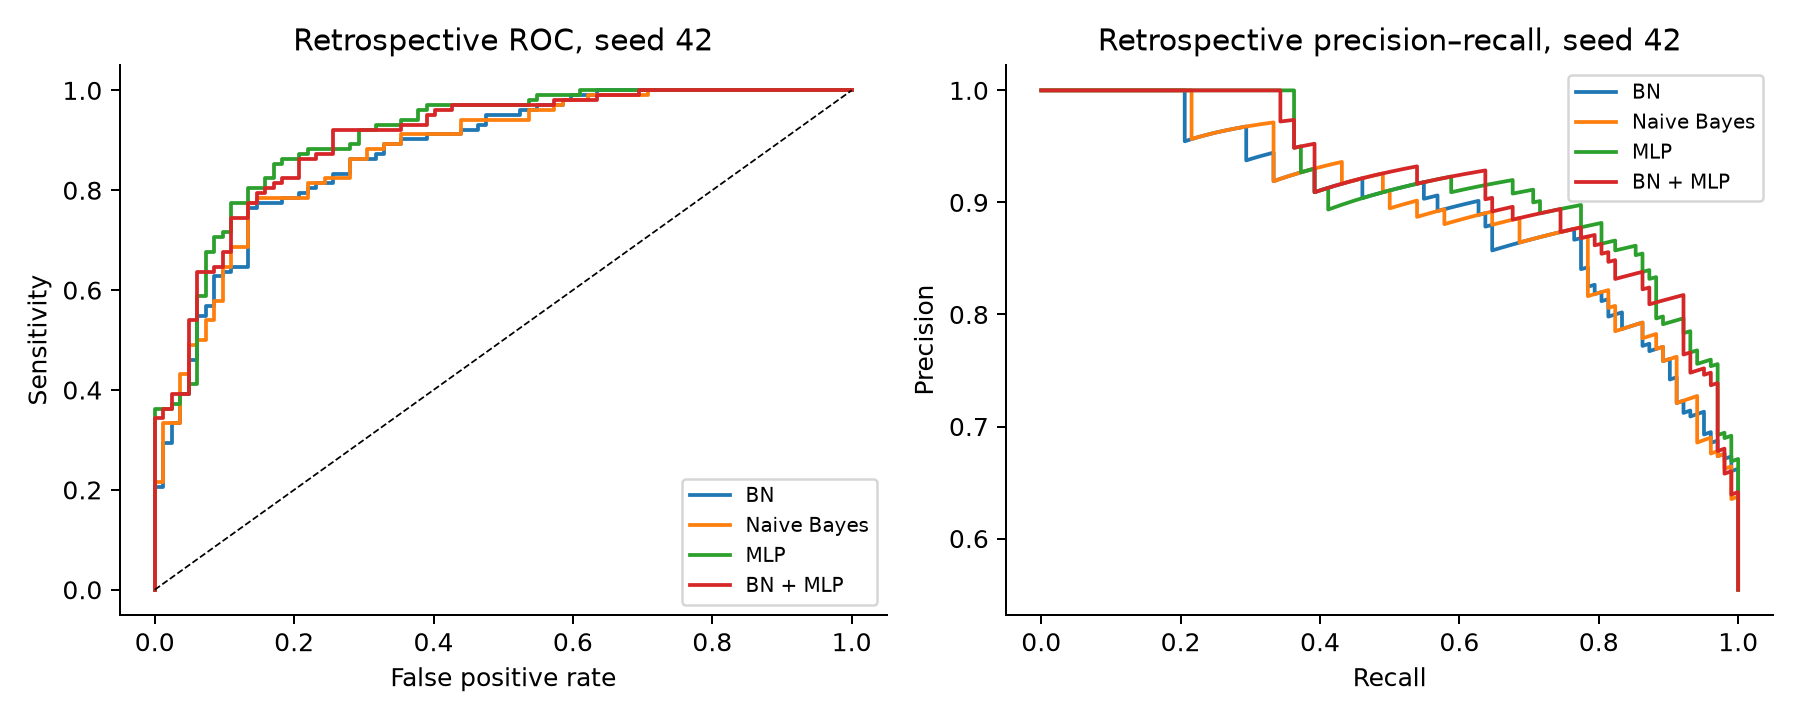
\includegraphics[width=\columnwidth]{../../artifacts/phase2/full_run/figures/discrimination.png}\caption{Seed-42 retrospective discrimination. Curves summarize this historical partition only.}\end{figure}
\begin{figure}[t]\centering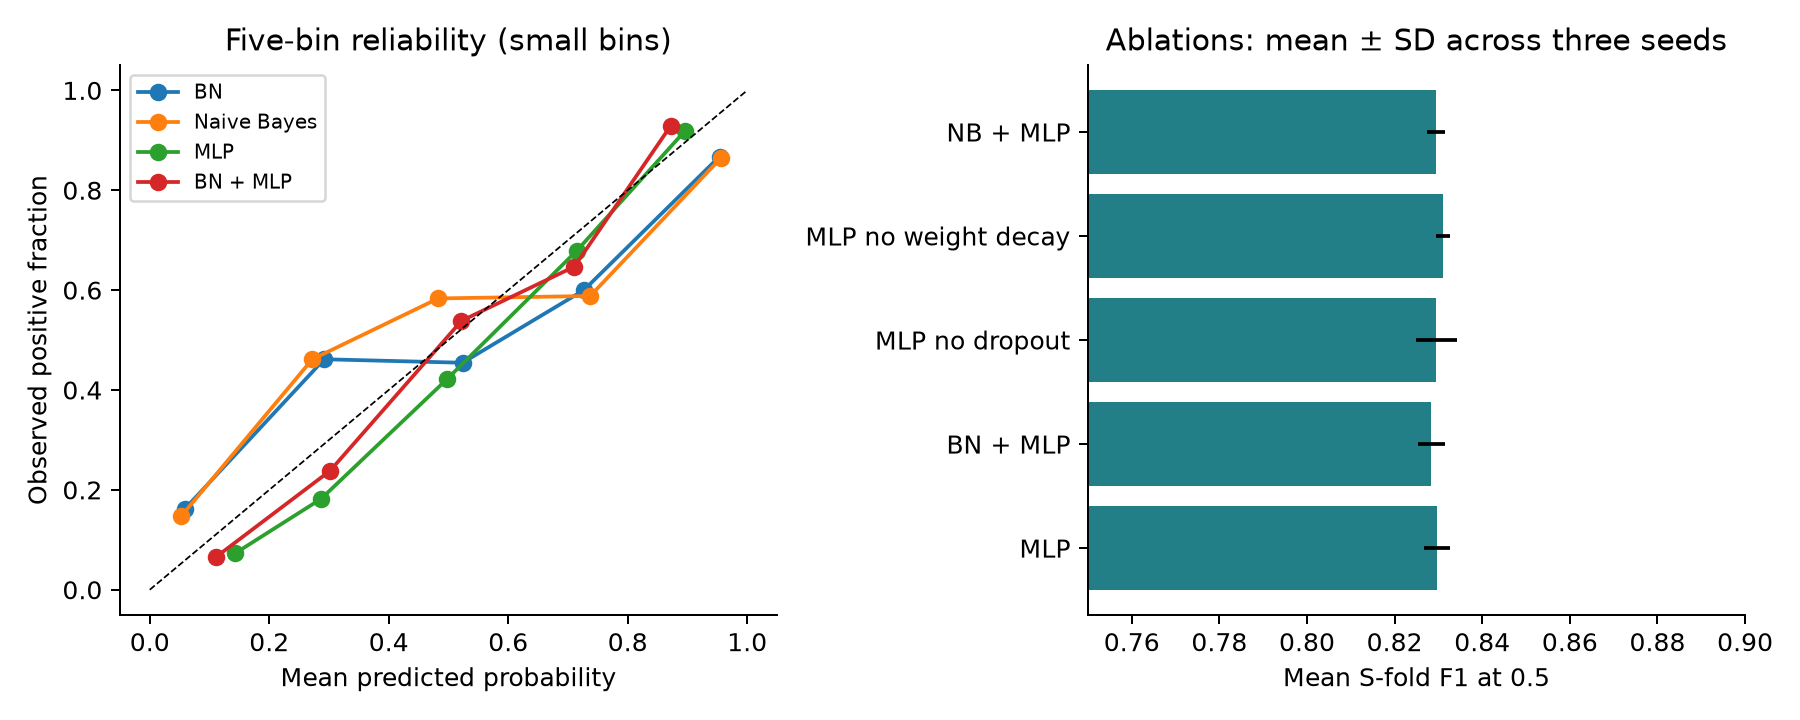
\includegraphics[width=\columnwidth]{../../artifacts/phase2/full_run/figures/calibration_ablations.png}\caption{Descriptive reliability and fixed-fold ablations. Error bars show standard deviation of seed-mean CV F1, not independent confidence intervals.}\end{figure}
\begin{figure}[t]\centering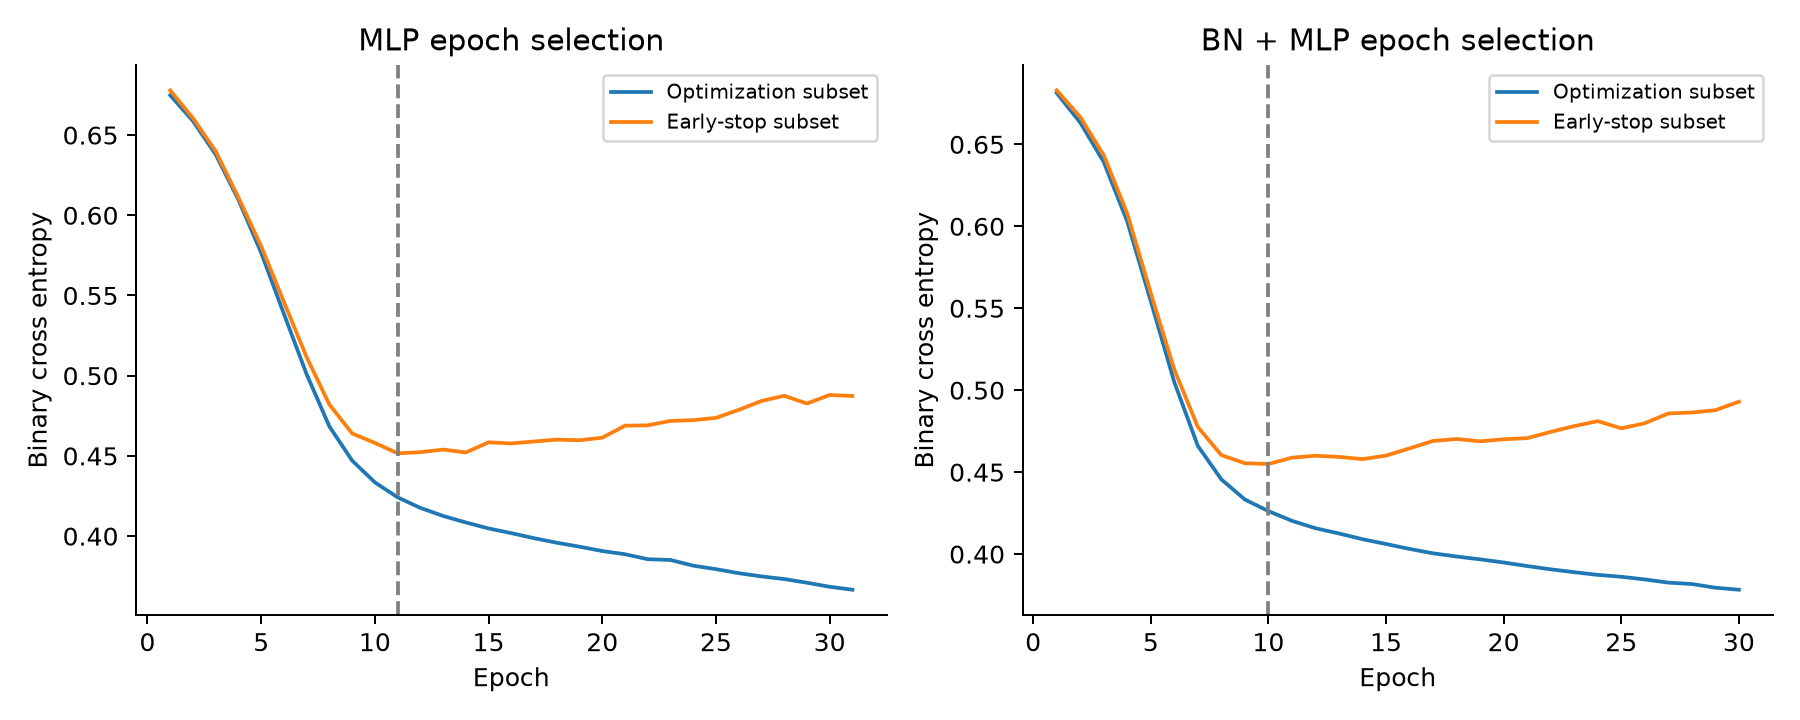
\includegraphics[width=\columnwidth]{../../artifacts/phase2/full_run/figures/learning_curves.png}\caption{Training-only epoch selection. Curves use the optimization and early-stop subsets within S, not T.}\end{figure}

Hospital transfer is uneven. MLP ROC-AUC is 0.8635 in Cleveland, 0.8791 in Hungary, 0.7372 in Switzerland and 0.5866 in VA Long Beach. The hybrid reaches 0.6930 in VA Long Beach, but specificity there remains 0.025 at its local cutoff, versus 0.050 for the MLP. A favorable AUC difference at one site does not demonstrate clinical utility or consistent hybrid value. Switzerland's high disease prevalence makes always-positive F1 a strong reference; saved site-level constant references must be consulted alongside model F1.
\section{Reproducibility and Technical Validation}
The repository includes a dedicated Phase 2 dependency specification and run-specific version lock, source and protocol hashes, exact partitions, common folds, every seed's predictions, training curves, early-stop and cross-fitting audits, BN states and cut points, frozen models, model hashes, cutoff searches and reconstructable metrics. The source CSV and AML artifacts are preserved.

The full-run verifier checks 35 saved models, including saved-model probability round trips, cutoff reconstruction, metric reconstruction, family selection, CV coverage and hospital isolation. Local testing passed 60 tests with 39 subtests; the unchanged Phase 1 Streamlit interface was excluded from this Phase 2 environment check. GitHub automation runs the dedicated Phase 2 tests and a smoke experiment on pushes. Smoke runs use three epochs and must never be cited as performance evidence.

The application-independent batch inference command accepts the eleven eligible predictors, verifies model integrity and uses the saved cutoff without fitting. The original Phase 1 web interface retains its own model evidence. Only trusted joblib files should be loaded.
\section{Limitations and Conclusions}
The experiment is small and retrospective, with uncertain patient linkage, incomplete merged-data provenance, hospital shifts and provisional graph assumptions. Row-level CV may exploit source-specific missingness. Calibration bins are sparse and descriptive. No prospective cohort, causal analysis, utility analysis or fairness validation is supplied.

The hybrid is a successful implementation of a testable hypothesis, but the measured results do not establish added value over the MLP. We therefore do not claim eligibility for performance-based hybrid bonus marks. The main deliverable is a transparent BN--MLP probability comparison with controlled preprocessing, ablations and reproducible evidence. Faculty approval of domain assumptions, correct individual contribution attribution, and the team's own presentation and viva remain essential.
\begin{thebibliography}{6}
\bibitem{pearl} J. Pearl, \emph{Probabilistic Reasoning in Intelligent Systems}. Morgan Kaufmann, 1988.
\bibitem{uci} A. Janosi, W. Steinbrunn, M. Pfisterer and R. Detrano, ``Heart Disease,'' UCI Machine Learning Repository, 1988. doi:10.24432/C52P4X.
\bibitem{gorishniy} Y. Gorishniy et al., ``Revisiting Deep Learning Models for Tabular Data,'' NeurIPS, 2021. arXiv:2106.11959.
\bibitem{grinsztajn} L. Grinsztajn, E. Oyallon and G. Varoquaux, ``Why do tree-based models still outperform deep learning on tabular data?'' NeurIPS, 2022. arXiv:2207.08815.
\bibitem{dropout} N. Srivastava et al., ``Dropout: A Simple Way to Prevent Neural Networks from Overfitting,'' JMLR, vol.15, pp.1929--1958, 2014.
\bibitem{guo} C. Guo et al., ``On Calibration of Modern Neural Networks,'' ICML, PMLR 70, pp.1321--1330, 2017.
\end{thebibliography}\end{document}
